\section{Formal Framework: Role Matrices, Ranking, and Superposition}
\label{sec:framework}

This section constructs the static state representations of \RST{} in four steps:
(1)~grounding functional roles inside a non-negative role matrix $M \in \Rnum_{\ge 0}^{n \times m}$
with zero-safe normalization and linear aggregation, (2)~comparing classical simplex
weights against complex Hilbert-space amplitudes and explicitly bounding the role of
complex phases, (3)~defining competition ordinal rank alongside Model~A
(\emph{DistributedWeights}) and Model~B (\emph{SharedMaximum}) to resolve the
sub-unit-weight flaw via $\mathbf{w} = (0.99, 0.01)$, and (4)~documenting reduced
partner density matrices and canonical worked examples.

\subsection{Role Basis, Raw Role Matrix, and Normalization}
\label{subsec:fw-primitives}

\begin{definition}[Relational role basis; \layerformal]
\label{def:role}
Let $\roleset = \{r_1, r_2, \dots, r_m\}$ be a finite set of distinct relational
functions ($m \ge 2$). In the canonical $5$-dimensional \RST{} basis:
\begin{align*}
  \roleset = \bigl\{&\text{primary visibility } (r_1),\, \text{emotional support } (r_2),\,
  \text{financial/material } (r_3), \\
  &\text{entertainment } (r_4),\, \text{contingency } (r_5)\bigr\}.
\end{align*}
In Hilbert-space coordinates, we associate $\roleset$ with an orthonormal basis
$\{\ket{r_1}, \dots, \ket{r_m}\}$ of $\vspaceR \cong \Cnum^m$ satisfying
$\braket{r_j}{r_\ell} = \delta_{j\ell}$. An extended $10$-role basis appears in \cref{app:roles}.
\end{definition}

\begin{table}[htbp]
\centering
\small
\caption{Canonical five-role basis $\roleset$ of Relational Superposition Theory.}
\label{tab:roles}
\begin{tabularx}{\textwidth}{@{}lllX@{}}
\toprule
Symbol & Relational role & Colloquial cue & Typical behavioral observables \\
\midrule
$r_1$ & Primary visibility & ``Main / official'' & Shared daytime social events, friends-group visibility \\
$r_2$ & Emotional support & ``The 2~a.m.\ listener'' & Late-night voice notes, stress venting, crisis processing \\
$r_3$ & Financial/material & ``Practical provider'' & Meals, rides, errands, logistical or financial favors \\
$r_4$ & Entertainment & ``Weekend energy'' & Parties, concerts, spontaneous outings, novelty \\
$r_5$ & Contingency reserve & ``Just in case'' & Low-cadence check-ins preserving reactivation potential \\
\bottomrule
\end{tabularx}
\end{table}

\noindent\layerformal{} To separate behavioral observations from Hilbert-space
abstractions, we begin with a finite partner set $\partnerset = \{G_1, \dots, G_n\}$
and a non-negative \emph{raw role matrix} $M \in \Rnum_{\ge 0}^{n \times m}$, whose entry
$M_{ij} \ge 0$ records partner $G_i$'s raw behavioral score on role $r_j$. Depending
on empirical or synthetic context, $M_{ij}$ represents normalized interaction counts,
weighted time-slot tallies, or rated rubric scores (\cref{app:instrument}).

\begin{definition}[Zero-safe column normalization and role dominance; \layerformal]
\label{def:role-matrix}
For each role column $j \in \{1, \dots, m\}$, let $S_j(M) = \sum_{i=1}^n M_{ij}$ denote
the total activity observed in role $r_j$. The \emph{column-normalized role matrix}
$\tilde{M} \in [0, 1]^{n \times m}$ is defined entrywise by
\begin{equation}
  \tilde{M}_{ij} =
  \begin{cases}
    \dfrac{M_{ij}}{S_j(M)} & \text{if } S_j(M) > 0, \\[8pt]
    0 & \text{if } S_j(M) = 0.
  \end{cases}
  \label{eq:col-normalize}
\end{equation}
Partner $G_i$ \emph{strictly dominates} role $r_j$ if $\tilde{M}_{ij} > \tilde{M}_{kj}$
for all $k \neq i$. Given a context weighting vector $\boldsymbol{\alpha} \in \Delta^{m-1}$,
each partner receives a scalar \emph{linear composite score}
\begin{equation}
  G_i(\boldsymbol{\alpha}) = \sum_{j=1}^{m} \alpha_j \tilde{M}_{ij},
  \qquad \text{with } 0 \le G_i(\boldsymbol{\alpha}) \le 1.
  \label{eq:global-score}
\end{equation}
\end{definition}

Zero-safe normalization avoids division-by-zero singularities when an optional role (such
as $r_3$) receives zero behavioral instances across all partners in a given window; both
the column-sum identity $\sum_i \tilde{M}_{ij} = 1$ (whenever $S_j > 0$) and the zero-column
guard are formally verified in \texttt{RST.Relational.RoleMatrix}. Importantly, because
$\tilde{M}$ is generally multi-peaked across columns, changing $\boldsymbol{\alpha}$ across
social contexts routinely reverses which partner attains $\max_i G_i(\boldsymbol{\alpha})$.

\begin{example}[Four-partner raw role matrix and aggregation rank reversal; \layerformal]
\label{ex:role-aggregation}
Consider the benchmark $4\times 5$ matrix used in Experiment~1 of \cref{sec:simulations}
(rows $G_1,\dots,G_4$, columns $r_1,\dots,r_5$):
\begin{equation*}
  M_{4\times 5} =
  \begin{pmatrix}
    8.5 & 3.0 & 2.0 & 3.5 & 1.0 \\
    2.5 & 9.0 & 1.5 & 2.0 & 1.5 \\
    1.5 & 2.0 & 8.8 & 1.8 & 2.0 \\
    1.5 & 1.8 & 1.2 & 8.2 & 4.5
  \end{pmatrix}.
\end{equation*}
$M_{4\times 5}$: column sums equal $(14.0,\, 15.8,\, 13.5,\, 15.5,\, 9.0)$ ($G_1$ leads
$r_1$, $G_2$ leads $r_2$, $G_3$ leads $r_3$, and $G_4$ leads $r_4, r_5$). Evaluating~\eqref{eq:global-score}
under public-visibility weights $\boldsymbol{\alpha}_{\mathrm{vis}} = (0.55, 0.15, 0.10, 0.15, 0.05)$
yields composite scores $(0.4167,\, 0.2225,\, 0.1716,\, 0.1893)$ ($G_1$ rank~$1$),
while support weights $\boldsymbol{\alpha}_{\mathrm{sup}} = (0.10, 0.50, 0.30, 0.05, 0.05)$
yield $(0.2169,\, 0.3508,\, 0.2865,\, 0.1458)$ ($G_2$ rank~$1$). Drawing $1{,}000$
uniform $\mathrm{Dir}(1,1,1,1,1)$ weights (\cref{fig:role-aggregation}) gives top-rank
counts $(227, 190, 253, 330)$ across $(G_1, G_2, G_3, G_4)$, proving every partner wins rank~$1$
on large simplex cones.
\end{example}

\begin{figure}[htbp]
  \centering
  \vspace{0.3em}
  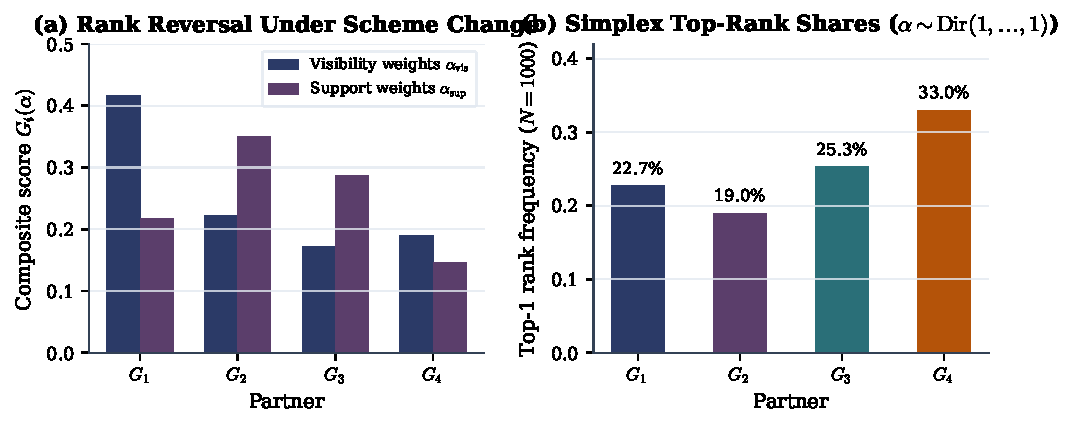
\includegraphics[width=0.98\textwidth]{figures/fig_role_aggregation.pdf}
  \caption{Synthetic linear aggregation sensitivity on $M_{4\times 5}$ (Seed \texttt{202605}).
  (a)~Rank reversal between $\boldsymbol{\alpha}_{\mathrm{vis}}$ ($G_1$ first at $0.4167$)
  and $\boldsymbol{\alpha}_{\mathrm{sup}}$ ($G_2$ first at $0.3508$). (b)~Top-1 share across
  $1{,}000$ uniform $\mathrm{Dir}(1,\dots,1)$ role weightings.}
  \label{fig:role-aggregation}
  \vspace{0.3em}
\end{figure}

\begin{definition}[Competition ordinal rank; \layermath]
\label{def:rank}
Given any non-negative partner weight vector $\mathbf{w} = (w_1, \dots, w_n) \in \Delta^{n-1}$
(with $w_i \ge 0$ and $\sum_{i=1}^n w_i = 1$), the \emph{competition ordinal rank} of partner
$G_i$ is defined without tie-breaking by
\begin{equation}
  r_i(\mathbf{w}) = 1 + \#\{j \in \{1, \dots, n\} : w_j > w_i\} \in \{1, \dots, n\}.
  \label{eq:ordinal-rank}
\end{equation}
Equal weights receive equal rank ($w_i = w_j \implies r_i(\mathbf{w}) = r_j(\mathbf{w})$),
and strictly dominated partners obey $r_i(\mathbf{w}) \ge 2$.
\end{definition}

\begin{definition}[Direct status inquiry / the poke; \layerbehav]
\label{def:poke}
A \emph{poke} is any intentional exogenous or partner-initiated intervention
$\poke$ forcing $W$ to resolve an ambiguity across rank or role (for instance, asking
``so what are we?'' or ``where do I stand relative to everyone else?'').
\end{definition}

\subsection{Classical Weight Vectors Versus Complex Hilbert-Space States}
\label{subsec:fw-states}

A central methodological question in \RST{} is how much vector machinery is strictly
needed. Two distinct formal representations coexist cleanly inside the model:

\begin{enumerate}[nosep]
  \item \textbf{Classical weight representation ($\Delta^{n-1}$).} Every static role
        profile, aggregate composite weight $w_i = G_i(\boldsymbol{\alpha}) / \sum_k G_k(\boldsymbol{\alpha})$,
        or Markovian attention occupancy vector lives in the classical probability simplex
        $\Delta^{n-1} = \{\mathbf{w} \in \Rnum_{\ge 0}^n : \sum_i w_i = 1\}$ (\texttt{Weights n}
        and \texttt{ProbDist n} in Lean~4). No complex numbers are required for ranking,
        normalization, or Markov transitions.
  \item \textbf{Complex Hilbert-space representation ($\vspaceTot = \vspaceG \otimes \vspaceR$).}
        To represent incompatible basis measurements in \cref{sec:uncertainty}, \RST{} lifts
        probabilities $w_i = \abs{a_i}^2$ and role fractions $p_{ij} = \abs{c_{ij}}^2$ to
        unit complex amplitude vectors in $\vspaceG \cong \Cnum^n$ and $\vspaceR \cong \Cnum^m$.
\end{enumerate}

\noindent\layerbehav{} \textbf{Honest scope of complex phases.} Complex relative phases
$\theta_i = \arg(a_i)$ are \emph{not} claimed to correspond to a directly measured
psychometric observable in human dating data. Within \RST{}, phases serve strictly as an
algebraic encoding of non-commuting context transformations $L = U(\gamma)^\dagger D_L U(\gamma)$
and phase-sensitive cross-terms inside inner products, reproducing classical simplex
statistics identically along diagonal bases ($\gamma = 0$).

\begin{definition}[Partner role-superposition state; \layerformal]
\label{def:partner-state}
For each partner $G_i \in \partnerset$, its \emph{role-superposition vector} in $\vspaceR$ is
\begin{equation}
  \ket{G_i} = \sum_{j=1}^{m} c_{ij} \ket{r_j},
  \qquad c_{ij} \in \Cnum,
  \qquad \sum_{j=1}^{m} \abs{c_{ij}}^2 = 1.
  \label{eq:partner-state}
\end{equation}
Here $p_{ij} = \abs{c_{ij}}^2$ represents partner $G_i$'s normalized share across role $r_j$,
matching the row-normalized counterpart of $M$. Partner $G_i$ is in a \emph{pure role} if
$\abs{c_{ij_0}}^2 = 1$ for a single $j_0$, and in a \emph{role superposition} if at least
two roles carry strictly positive weight.
\end{definition}

\begin{definition}[Composite relational system state; \layerformal]
\label{def:system-state}
Let $\{\ket{e_1}, \dots, \ket{e_n}\}$ be an orthonormal basis indexing partner identities
in $\vspaceG \cong \Cnum^n$, and let $a_1, \dots, a_n \in \Cnum$ satisfy
$\sum_{i=1}^n \abs{a_i}^2 = 1$. The \emph{composite relational system state} in
$\vspaceTot = \vspaceG \otimes \vspaceR \cong \Cnum^{nm}$ is
\begin{equation}
  \ket{\Psi} = \sum_{i=1}^{n} a_i \bigl(\ket{e_i} \otimes \ket{G_i}\bigr)
  = \sum_{i=1}^{n} \sum_{j=1}^{m} a_i c_{ij}\, \ket{e_i} \otimes \ket{r_j},
  \label{eq:system-state}
\end{equation}
with partner primary weight $w_i = \abs{a_i}^2 \ge 0$ satisfying $\sum_{i=1}^n w_i = 1$.
\end{definition}

\begin{lemma}[Unit normalization of composite state; \layermath]
\label{lem:composite-norm}
If $\sum_{i=1}^n \abs{a_i}^2 = 1$ and $\sum_{j=1}^m \abs{c_{ij}}^2 = 1$ for each $i$, then
$\ket{\Psi}$ in~\eqref{eq:system-state} has unit norm:
\begin{equation}
  \braket{\Psi}{\Psi} = \sum_{i=1}^{n} \sum_{j=1}^{m} \abs{a_i c_{ij}}^2 = 1.
  \label{eq:composite-norm}
\end{equation}
\end{lemma}
\begin{proof}
By orthonormality $\braket{e_i \otimes r_j}{e_k \otimes r_\ell} = \delta_{ik}\delta_{j\ell}$,
$\braket{\Psi}{\Psi} = \sum_{i=1}^n \abs{a_i}^2 \sum_{j=1}^m \abs{c_{ij}}^2 = \sum_{i=1}^n \abs{a_i}^2 = 1$.
\end{proof}

\subsection{Distributed Weights Versus Shared Maxima: Resolving the Central Flaw}
\label{subsec:fw-superposition}

The initial (v1.0) formulation of \RST{} defined relational superposition solely by the
presence of at least two positively weighted partners ($w_i > 0, w_j > 0$ for $i \neq j$)
and claimed that this precluded any partner from holding rank~$1$. As a mathematical claim,
that inference is false.

\begin{example}[The $\mathbf{w} = (0.99, 0.01)$ counterexample; \layerformal]
\label{ex:w99-counterexample}
Consider $n = 2$ partners with weight vector $\mathbf{w}_{99} = (0.99, 0.01)$. Both entries
are strictly positive and strictly below $1$, so weight is distributed across two partners.
Evaluating~\eqref{eq:ordinal-rank}, however, gives $r_1(\mathbf{w}_{99}) = 1$ and
$r_2(\mathbf{w}_{99}) = 2$: partner $G_1$ holds a unique global maximum ($\forall j \neq 1,\;
w_j < w_1$). Distributed weights exclude monopoly ($w_k = 1$), not ordinal dominance.
\end{example}

To state what distributed weights do and do not imply cleanly, we distinguish two formal
predicates over any weight vector $\mathbf{w} \in \Delta^{n-1}$:

\begin{definition}[Model~A vs.\ Model~B rank-indeterminacy predicates; \layerformal]
\label{def:superposition}
Let $\mathbf{w} \in \Delta^{n-1}$ be a normalized partner weight vector ($w_i = \abs{a_i}^2$).
\begin{enumerate}[nosep]
  \item \emph{Unique maximum}: partner $G_k$ holds a \emph{unique maximum} if
        $w_j < w_k$ for all $j \neq k$.
  \item \emph{Model~A (\textnormal{\texttt{DistributedWeights}})}: there exist distinct
        $i \neq j$ with $w_i > 0$ and $w_j > 0$.
  \item \emph{Model~B (\textnormal{\texttt{SharedMaximum}})}: there exist distinct
        $i \neq j$ such that $w_k \le w_i$ and $w_k \le w_j$ for all $k \in \{1, \dots, n\}$
        (or within a near-tie indistinguishability band $\abs{\max_k w_k - w_i} \le \epsilon$).
\end{enumerate}
Under strong \RST{} indeterminacy prior to context selection, either Model~B holds on
aggregate attention weights or distinct contexts $\boldsymbol{\alpha}$ induce incompatible
ordinal maximizers (\cref{ex:role-aggregation}).
\end{definition}

\begin{proposition}[Precise scope of sub-unit weight versus shared-maximum rank; \layerformal]
\label{prop:nobody-first}
For any weight vector $\mathbf{w} \in \Delta^{n-1}$ ($n \ge 2$):
\begin{enumerate}[nosep]
  \item \textbf{Model~A scope:} If \textnormal{\texttt{DistributedWeights}}$(\mathbf{w})$ holds,
        then $w_k < 1$ for every $k \in \{1, \dots, n\}$ (no partner holds all relational weight).
  \item \textbf{Model~B excludes unique rank~1:} If \textnormal{\texttt{SharedMaximum}}$(\mathbf{w})$
        holds, then no partner satisfies \textnormal{\texttt{UniqueMaximum}}, and at least two
        distinct partners attain competition ordinal rank $r_i(\mathbf{w}) = r_j(\mathbf{w}) = 1$.
  \item \textbf{Non-implication:} \textnormal{\texttt{DistributedWeights}}$(\mathbf{w})$ does
        \emph{not} imply \textnormal{\texttt{SharedMaximum}}$(\mathbf{w})$, as witnessed by
        $\mathbf{w}_{99} = (99/100, 1/100)$.
\end{enumerate}
\end{proposition}
\begin{proof}
For~(1), if $w_i, w_j > 0$ with $i \neq j$, then for any index $k$ at least one of $i, j$
differs from $k$, whence $w_k \le 1 - w_{\ell} < 1$ where $\ell \in \{i,j\}\setminus\{k\}$.
For~(2), if $i \neq j$ both attain $\max_t w_t$, neither can be strictly exceeded nor can any
single $k$ satisfy $w_i < w_k$ and $w_j < w_k$ simultaneously; hence $\#\{t : w_t > w_i\} = 0$,
yielding $r_i = r_j = 1$. Statement~(3) follows immediately from \cref{ex:w99-counterexample}.
Every part of \cref{prop:nobody-first} is formally proved in \texttt{RST.Relational.SharedMaximum}.
\end{proof}

\noindent\layerbehav{} Operationally, $\mathbf{w}_{99}$ characterizes a near-exclusive
commitment retaining a single low-cadence acquaintance on the side. Only Model~B,
or context-driven rank reversal across a non-dominated role matrix $M$, captures
an arrangement in which no participant holds an undisputed rank~$1$.

\subsection{Matrix Visualization and Entropy Measures}
\label{subsec:fw-matrix}

Putting partner weights $w_i = \abs{a_i}^2$ together with normalized role profiles
$p_{ij} = \abs{c_{ij}}^2$ yields the $n \times m$ weighted joint partner-role matrix $W$
with entries $W_{ij} = w_i p_{ij}$ and $\sum_{i,j} W_{ij} = 1$. Marginalizing over partners
gives aggregate system coverage of role $r_j$:
\begin{equation}
  \bar{p}_j = \sum_{i=1}^{n} w_i p_{ij} = \sum_{i=1}^{n} \abs{a_i c_{ij}}^2.
  \label{eq:marginal-role}
\end{equation}
\cref{fig:weight-matrix} illustrates a $4$-partner portfolio partitioned across the five
canonical roles.

\begin{figure}[htbp]
  \centering
  \vspace{0.3em}
  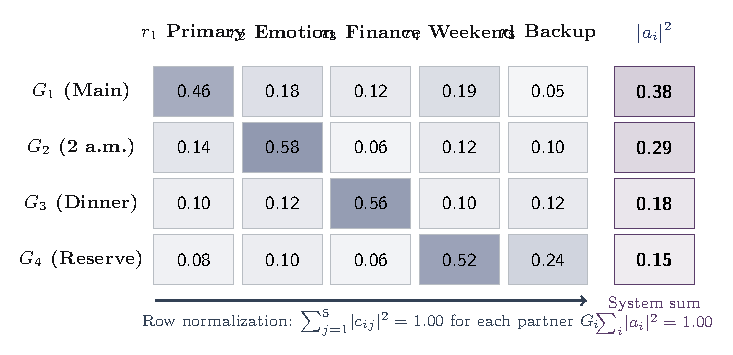
\includegraphics[width=0.95\textwidth]{figures/fig_weight_matrix.pdf}
  \caption{Partner-role matrix visualization for a $4$-partner portfolio. Left: conditional
  role probabilities $p_{ij} = \abs{c_{ij}}^2$ alongside partner attention shares $w_i = \abs{a_i}^2$.
  Right: joint relational probability mass $W_{ij} = w_i p_{ij}$.}
  \label{fig:weight-matrix}
  \vspace{0.3em}
\end{figure}

\begin{definition}[Rank entropy and role entropy; \layermath]
\label{def:entropies}
Using Shannon entropy in bits~\citep{shannon1948mathematical,cover2006elements} with
$0 \log_2 0 \equiv 0$, the \emph{system rank entropy} $H(\mathbf{w})$ and the
\emph{conditional role entropy} $H(R \mid G)$ are
\begin{equation}
  H(\mathbf{w}) = -\sum_{i=1}^{n} w_i \log_2 w_i,
  \qquad
  H(R \mid G) = -\sum_{i=1}^{n} w_i \sum_{j=1}^{m} p_{ij} \log_2 p_{ij}.
  \label{eq:entropies}
\end{equation}
\end{definition}

When $\mathbf{w}$ concentrates on a single collapsed partner, $H(\mathbf{w}) = 0$. Under
uniform weights $w_i = 1/n$, $H(\mathbf{w}) = \log_2 n$.

\subsection{Pure States Versus Mixed Density Operators}
\label{subsec:fw-density}

Tracing out the partner register from $\rho_{\mathrm{tot}} = \ketbra{\Psi}{\Psi}$ yields
the reduced role density matrix $\rho_R = \operatorname{tr}_G(\rho_{\mathrm{tot}}) =
\sum_{i=1}^n \abs{a_i}^2 \ketbra{G_i}{G_i}$ with no partner cross-terms; conversely,
tracing out $\vspaceR$ yields the reduced partner density matrix
\begin{equation}
  (\rho_G)_{ik} = a_i a_k^* \braket{G_k}{G_i}
  = a_i a_k^* \sum_{j=1}^{m} c_{kj}^* c_{ij}.
  \label{eq:reduced-partner-rho}
\end{equation}
When partners have disjoint roles ($\braket{G_k}{G_i} = \delta_{ik}$), $\rho_G$ reduces to
a classical diagonal mixture $\diag(w_1, \dots, w_n)$ of rank~1 projectors; whenever roles
overlap ($\braket{G_k}{G_i} \neq 0$), off-diagonal coherences persist prior to collapse.

\begin{example}[Pure coherent state vs.\ maximally mixed portfolio; \layermath]
\label{ex:density-comparison}
Consider $n = 2$ partners sharing identical role profile $\ket{G_1} = \ket{G_2} = \ket{r_2}$
with equal weights $w_1 = w_2 = 1/2$. In the coherent pure state $\ket{\Psi_+} =
\frac{1}{\sqrt{2}}(\ket{e_1} + \ket{e_2})\otimes\ket{r_2}$,
$\rho_{G,\mathrm{pure}} = \frac{1}{2}\begin{psmallmatrix} 1 & 1 \\ 1 & 1 \end{psmallmatrix}$
satisfies $\operatorname{tr}(\rho^2) = 1$, whereas the incoherent statistical mixture
$\rho_{G,\mathrm{mix}} = \frac{1}{2}\begin{psmallmatrix} 1 & 0 \\ 0 & 1 \end{psmallmatrix}$
satisfies $\operatorname{tr}(\rho^2) = 1/2$, while both produce identical marginal selection
odds $(1/2, 1/2)$ under a partner-identity poke.
\end{example}

\subsection{Canonical Numerical Examples}
\label{subsec:fw-examples}

\begin{example}[Symmetric three-partner role partition (Triad); \layerformal]
\label{ex:triad}
Let $n = 3$, $m = 3$ with uniform system weights $w_i = 1/3$ ($a_i = 1/\sqrt{3}$) satisfying
\textnormal{\texttt{SharedMaximum}}, and role profiles $\ket{G_1} = \sqrt{0.85}\ket{r_1} + \sqrt{0.15}\ket{r_4}$,
$\ket{G_2} = \sqrt{0.90}\ket{r_2} + \sqrt{0.10}\ket{r_5}$, and
$\ket{G_3} = \sqrt{0.85}\ket{r_3} + \sqrt{0.15}\ket{r_4}$. Then $H(\mathbf{w}) = \log_2 3 \approx 1.585$~bits,
every partner ties at competition rank~$1$, and aggregate coverage is
$\bar{\mathbf{p}} = (0.283, 0.300, 0.283, 0.100, 0.033)$.
\end{example}

\begin{example}[Asymmetric four-partner portfolio (Quartet); \layerformal]
\label{ex:quartet}
Let $\mathbf{w} = (0.34, 0.28, 0.22, 0.16)$ match the initial vector of Experiment~2
in \cref{sec:simulations}, giving $H(\mathbf{w}) \approx 1.946$~bits. Here $G_1$ has the
largest single scalar attention share ($0.34 < 1$), placing this static snapshot in
Model~A rather than Model~B; genuine rank ambiguity arises as context weights shift across
days (\cref{sec:dynamics}) or across role schemes (\cref{ex:role-aggregation}).
\end{example}
